% ============================================================
% Chapitre 4 : R\'egularisation -- Ridge, Lasso, Elastic Net
% ============================================================
\chapter{R\'egularisation --- Ridge, Lasso, Elastic Net}
\label{ch:regularisation}

\begin{intuition}[title=\textbf{Pourquoi r\'egulariser ?}]
Un mod\`ele trop complexe (trop de param\`etres, degr\'e polynomial \'elev\'e)
s'ajuste parfaitement aux donn\'ees d'entra\^inement mais g\'en\'eralise mal :
c'est le \textbf{sur-apprentissage}. La r\'egularisation ajoute un terme de
p\'enalit\'e \`a la fonction de co\^ut pour contraindre la norme des coefficients
et ainsi contr\^oler la complexit\'e du mod\`ele.
\end{intuition}

% ============================================================
\section{Le probl\`eme du sur-apprentissage}
\label{sec:overfitting}

\begin{definition}[D\'ecomposition biais-variance]
Pour un mod\`ele $\hat{f}$ appris sur un \'echantillon al\'eatoire, l'erreur de
g\'en\'eralisation en un point $\bm{x}_0$ se d\'ecompose en :
\[
  \E\bigl[(y_0 - \hat{f}(\bm{x}_0))^2\bigr]
  = \underbrace{\Bias(\hat{f}(\bm{x}_0))^2}_{\text{erreur syst\'ematique}}
  + \underbrace{\Var(\hat{f}(\bm{x}_0))}_{\text{instabilit\'e}}
  + \underbrace{\sigma^2}_{\text{bruit irr\'eductible}}
\]
o\`u $\Bias(\hat{f}(\bm{x}_0)) = \E[\hat{f}(\bm{x}_0)] - f(\bm{x}_0)$.
\end{definition}

\begin{attention}[title=\textbf{Compromis biais-variance}]
\begin{itemize}
  \item \textbf{Mod\`ele trop simple} (sous-apprentissage) : biais \'elev\'e, variance faible.
  \item \textbf{Mod\`ele trop complexe} (sur-apprentissage) : biais faible, variance \'elev\'ee.
  \item La r\'egularisation \textbf{augmente l\'eg\`erement le biais} pour
        \textbf{r\'eduire fortement la variance}, ce qui am\'eliore l'erreur totale.
\end{itemize}
\end{attention}

\begin{formules}[title=\textbf{Cadre g\'en\'eral de r\'egularisation}]
On minimise la fonction de co\^ut r\'egularis\'ee :
\[
  \hat{\bm{\beta}} = \argmin_{\bm{\beta}} \left\{
    \frac{1}{n}\norm{\bm{y} - \bm{X}\bm{\beta}}^2 + \lambda \cdot \Omega(\bm{\beta})
  \right\}
\]
o\`u $\lambda \geq 0$ est l'\textbf{hyperparam\`etre de r\'egularisation} et
$\Omega(\bm{\beta})$ est la fonction de p\'enalit\'e.
\end{formules}

% ============================================================
\section{R\'egression Ridge (p\'enalit\'e $\ell_2$)}
\label{sec:ridge}

\subsection{Formulation}

\begin{definition}[R\'egression Ridge]
La r\'egression Ridge (Hoerl \& Kennard, 1970) utilise la p\'enalit\'e $\ell_2$ :
\[
  \hat{\bm{\beta}}_{\text{Ridge}} = \argmin_{\bm{\beta}} \left\{
    \norm{\bm{y} - \bm{X}\bm{\beta}}^2 + \lambda \norm{\bm{\beta}}^2_2
  \right\}
\]
o\`u $\norm{\bm{\beta}}_2^2 = \sum_{j=1}^{p} \beta_j^2$ (le biais $\beta_0$ n'est
g\'en\'eralement pas p\'enalis\'e).
\end{definition}

\subsection{Solution en forme ferm\'ee}

\begin{theoreme}[Solution Ridge]
\label{thm:ridge-solution}
La solution de la r\'egression Ridge est :
\[
  \hat{\bm{\beta}}_{\text{Ridge}} = (\bm{X}^\top \bm{X} + \lambda \bm{I}_p)^{-1}\bm{X}^\top \bm{y}
\]
Cette solution existe toujours, m\^eme si $\bm{X}^\top \bm{X}$ est singuli\`ere.
\end{theoreme}

\begin{proof}
La fonction de co\^ut Ridge s'\'ecrit :
\[
  \mathcal{L}_{\text{Ridge}}(\bm{\beta})
  = (\bm{y} - \bm{X}\bm{\beta})^\top(\bm{y} - \bm{X}\bm{\beta})
  + \lambda \bm{\beta}^\top \bm{\beta}
\]
Le gradient est :
\[
  \nabla_{\bm{\beta}} \mathcal{L}_{\text{Ridge}}
  = -2\bm{X}^\top(\bm{y} - \bm{X}\bm{\beta}) + 2\lambda \bm{\beta}
  = -2\bm{X}^\top \bm{y} + 2(\bm{X}^\top \bm{X} + \lambda \bm{I}_p)\bm{\beta}
\]
En annulant ce gradient :
\[
  (\bm{X}^\top \bm{X} + \lambda \bm{I}_p)\hat{\bm{\beta}} = \bm{X}^\top \bm{y}
\]
La matrice $\bm{X}^\top \bm{X} + \lambda \bm{I}_p$ est d\'efinie positive pour
$\lambda > 0$ (ses valeurs propres sont $\sigma_j^2 + \lambda > 0$), donc inversible.
\end{proof}

\subsection{Interpr\'etation par d\'ecomposition en valeurs singuli\`eres}

\begin{proposition}[Ridge et SVD]
\label{prop:ridge-svd}
Si $\bm{X} = \bm{U}\bm{\Sigma}\bm{V}^\top$ est la SVD de $\bm{X}$, avec
$\sigma_1 \geq \cdots \geq \sigma_p$ les valeurs singuli\`eres, alors :
\[
  \hat{\bm{y}}_{\text{Ridge}} = \bm{X}\hat{\bm{\beta}}_{\text{Ridge}}
  = \sum_{j=1}^{p} \frac{\sigma_j^2}{\sigma_j^2 + \lambda} \inner{\bm{u}_j}{\bm{y}} \bm{u}_j
\]
Le facteur $\frac{\sigma_j^2}{\sigma_j^2 + \lambda} \in [0, 1)$ \textbf{r\'etr\'ecit}
les composantes associ\'ees aux petites valeurs singuli\`eres.
\end{proposition}

\subsection{Interpr\'etation bay\'esienne}

\begin{theoreme}[Ridge comme estimateur MAP]
Si $\bm{\beta} \sim \mathcal{N}(\bm{0}, \tau^2 \bm{I}_p)$ a priori et
$\bm{y} \mid \bm{\beta} \sim \mathcal{N}(\bm{X}\bm{\beta}, \sigma^2 \bm{I}_n)$,
alors l'estimateur du \textbf{maximum a posteriori} (MAP) est :
\[
  \hat{\bm{\beta}}_{\text{MAP}} = \argmax_{\bm{\beta}} P(\bm{\beta} \mid \bm{y})
  = (\bm{X}^\top \bm{X} + \frac{\sigma^2}{\tau^2}\bm{I}_p)^{-1}\bm{X}^\top \bm{y}
  = \hat{\bm{\beta}}_{\text{Ridge}}
\]
avec $\lambda = \sigma^2 / \tau^2$.
\end{theoreme}

\begin{proof}
Par le th\'eor\`eme de Bayes, $P(\bm{\beta} \mid \bm{y}) \propto P(\bm{y} \mid \bm{\beta})P(\bm{\beta})$.
En prenant le logarithme :
\begin{align*}
  \log P(\bm{\beta} \mid \bm{y})
  &= \text{const} - \frac{1}{2\sigma^2}\norm{\bm{y} - \bm{X}\bm{\beta}}^2
     - \frac{1}{2\tau^2}\norm{\bm{\beta}}^2 \\
  &= \text{const} - \frac{1}{2\sigma^2}\left[
     \norm{\bm{y} - \bm{X}\bm{\beta}}^2 + \frac{\sigma^2}{\tau^2}\norm{\bm{\beta}}^2
  \right]
\end{align*}
Maximiser revient \`a minimiser le crit\`ere Ridge avec $\lambda = \sigma^2/\tau^2$.
\end{proof}

% ============================================================
\section{R\'egression Lasso (p\'enalit\'e $\ell_1$)}
\label{sec:lasso}

\subsection{Formulation}

\begin{definition}[R\'egression Lasso]
Le Lasso (\emph{Least Absolute Shrinkage and Selection Operator}, Tibshirani 1996)
utilise la p\'enalit\'e $\ell_1$ :
\[
  \hat{\bm{\beta}}_{\text{Lasso}} = \argmin_{\bm{\beta}} \left\{
    \frac{1}{2n}\norm{\bm{y} - \bm{X}\bm{\beta}}^2 + \lambda \norm{\bm{\beta}}_1
  \right\}
\]
o\`u $\norm{\bm{\beta}}_1 = \sum_{j=1}^{p} |\beta_j|$.
\end{definition}

\begin{attention}[title=\textbf{Pas de solution analytique}]
La p\'enalit\'e $\ell_1$ n'est pas diff\'erentiable en $\beta_j = 0$. Il n'existe pas
de solution en forme ferm\'ee. On utilise des algorithmes sp\'ecifiques : descente de
coordonn\'ees, ISTA/FISTA, LARS, etc.
\end{attention}

\subsection{Parcimonie et s\'election de variables}

\begin{theoreme}[Parcimonie du Lasso]
Le Lasso produit des solutions \textbf{parcimonieuses} : pour $\lambda$ suffisamment
grand, certains coefficients $\hat{\beta}_j$ sont \emph{exactement} nuls.
Le Lasso r\'ealise ainsi une \textbf{s\'election automatique de variables}.
\end{theoreme}

\begin{lemme}[Op\'erateur de seuillage doux]
\label{lem:soft-threshold}
Pour le probl\`eme unidimensionnel
$\min_{\beta} \frac{1}{2}(\beta - z)^2 + \lambda|\beta|$,
la solution est l'op\'erateur de \textbf{seuillage doux} (\emph{soft thresholding}) :
\[
  \hat{\beta} = S_\lambda(z) = \text{sign}(z)\max(|z| - \lambda, 0)
  = \begin{cases}
    z - \lambda & \text{si } z > \lambda \\
    0 & \text{si } |z| \leq \lambda \\
    z + \lambda & \text{si } z < -\lambda
  \end{cases}
\]
\end{lemme}

\subsection{Interpr\'etation g\'eom\'etrique}

\begin{intuition}[title=\textbf{Pourquoi $\ell_1$ produit des z\'eros et pas $\ell_2$}]
La formulation contrainte \'equivalente est :
\[
  \min_{\bm{\beta}} \norm{\bm{y} - \bm{X}\bm{\beta}}^2
  \quad \text{sous} \quad \norm{\bm{\beta}}_q \leq t
\]
avec $q = 1$ (Lasso) ou $q = 2$ (Ridge). En 2D, la r\'egion $\norm{\bm{\beta}}_1 \leq t$
est un \textbf{losange} dont les sommets sont sur les axes, tandis que
$\norm{\bm{\beta}}_2 \leq t$ est un \textbf{disque}. Les courbes de niveau
elliptiques de $\mathcal{L}$ ont tendance \`a toucher le losange en un sommet (donc
un coefficient nul), mais le disque en un point g\'en\'erique.
\end{intuition}

% --- TikZ : r\'egions de contrainte L1 / L2 ---
\begin{figure}[htbp]
\centering
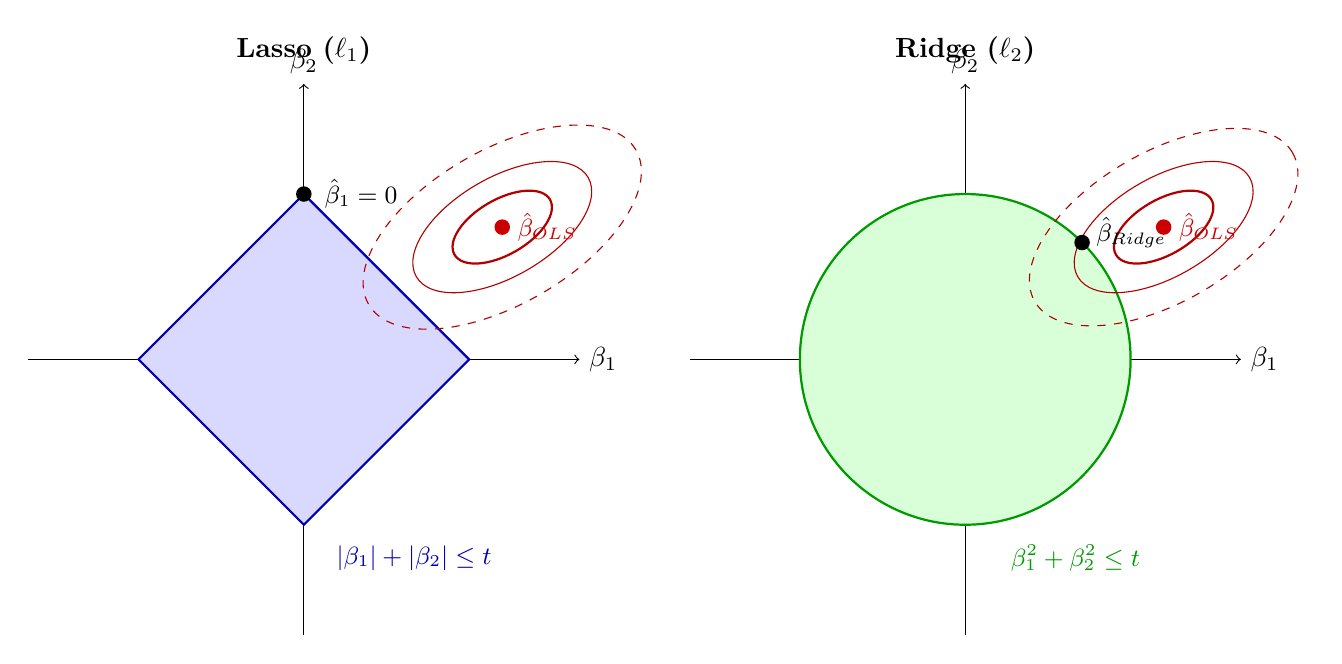
\begin{tikzpicture}[scale=1.4]
  % --- Lasso (L1) ---
  \begin{scope}[xshift=0cm]
    \node[font=\bfseries] at (0, 2.8) {Lasso ($\ell_1$)};
    \draw[->] (-2.5,0) -- (2.5,0) node[right]{$\beta_1$};
    \draw[->] (0,-2.5) -- (0,2.5) node[above]{$\beta_2$};
    % losange L1
    \fill[blue!15] (1.5,0) -- (0,1.5) -- (-1.5,0) -- (0,-1.5) -- cycle;
    \draw[thick, blue!70!black] (1.5,0) -- (0,1.5) -- (-1.5,0) -- (0,-1.5) -- cycle;
    \node[blue!70!black, font=\small] at (1.0, -1.8) {$|\beta_1|+|\beta_2| \leq t$};
    % ellipses de niveau
    \draw[red!70!black, thick, rotate around={30:(1.8,1.2)}]
      (1.8,1.2) ellipse (0.5 and 0.25);
    \draw[red!70!black, rotate around={30:(1.8,1.2)}]
      (1.8,1.2) ellipse (0.9 and 0.45);
    \draw[red!70!black, dashed, rotate around={30:(1.8,1.2)}]
      (1.8,1.2) ellipse (1.4 and 0.7);
    % point de tangence sur l'axe
    \fill[black] (0, 1.5) circle (2pt);
    \node[right, font=\small] at (0.1, 1.5) {$\hat{\beta}_1 = 0$};
    % OLS
    \fill[red!80!black] (1.8, 1.2) circle (2pt);
    \node[right, red!80!black, font=\small] at (1.85, 1.2) {$\hat{\beta}_{\text{OLS}}$};
  \end{scope}
  % --- Ridge (L2) ---
  \begin{scope}[xshift=6cm]
    \node[font=\bfseries] at (0, 2.8) {Ridge ($\ell_2$)};
    \draw[->] (-2.5,0) -- (2.5,0) node[right]{$\beta_1$};
    \draw[->] (0,-2.5) -- (0,2.5) node[above]{$\beta_2$};
    % disque L2
    \fill[green!15] (0,0) circle (1.5);
    \draw[thick, green!60!black] (0,0) circle (1.5);
    \node[green!60!black, font=\small] at (1.0, -1.8) {$\beta_1^2+\beta_2^2 \leq t$};
    % ellipses de niveau
    \draw[red!70!black, thick, rotate around={30:(1.8,1.2)}]
      (1.8,1.2) ellipse (0.5 and 0.25);
    \draw[red!70!black, rotate around={30:(1.8,1.2)}]
      (1.8,1.2) ellipse (0.9 and 0.45);
    \draw[red!70!black, dashed, rotate around={30:(1.8,1.2)}]
      (1.8,1.2) ellipse (1.35 and 0.68);
    % point de tangence generique
    \fill[black] (1.06, 1.06) circle (2pt);
    \node[right, font=\small] at (1.1, 1.15) {$\hat{\beta}_{\text{Ridge}}$};
    % OLS
    \fill[red!80!black] (1.8, 1.2) circle (2pt);
    \node[right, red!80!black, font=\small] at (1.85, 1.2) {$\hat{\beta}_{\text{OLS}}$};
  \end{scope}
\end{tikzpicture}
\caption{Interpr\'etation g\'eom\'etrique : la r\'egion $\ell_1$ (losange) favorise les solutions
parcimonieuses (sommets sur les axes), contrairement \`a la r\'egion $\ell_2$ (disque).}
\label{fig:l1-l2-constraint}
\end{figure}

\subsection{Interpr\'etation bay\'esienne du Lasso}

\begin{remarque}
Le Lasso correspond \`a un a priori de Laplace sur les coefficients :
$\beta_j \sim \text{Laplace}(0, b)$ avec $p(\beta_j) = \frac{1}{2b}\exp(-|\beta_j|/b)$.
L'estimateur MAP donne le Lasso avec $\lambda = \sigma^2 / (nb)$.
Contrairement au prior gaussien (Ridge), le prior de Laplace concentre plus de masse
en z\'ero, ce qui explique la parcimonie.
\end{remarque}

% ============================================================
\section{Elastic Net}
\label{sec:elastic-net}

\begin{definition}[Elastic Net]
L'Elastic Net (Zou \& Hastie, 2005) combine les p\'enalit\'es $\ell_1$ et $\ell_2$ :
\[
  \hat{\bm{\beta}}_{\text{EN}} = \argmin_{\bm{\beta}} \left\{
    \frac{1}{2n}\norm{\bm{y} - \bm{X}\bm{\beta}}^2
    + \lambda \Bigl[\alpha \norm{\bm{\beta}}_1 + \frac{1-\alpha}{2}\norm{\bm{\beta}}_2^2\Bigr]
  \right\}
\]
o\`u $\alpha \in [0, 1]$ contr\^ole le m\'elange ($\alpha = 1$ : Lasso pur,
$\alpha = 0$ : Ridge pur).
\end{definition}

\begin{bonnepratique}[title=\textbf{Quand utiliser l'Elastic Net}]
\begin{itemize}
  \item Quand $p > n$ (plus de variables que d'observations), le Lasso s\'electionne
        au plus $n$ variables. L'Elastic Net n'a pas cette limitation.
  \item Quand des variables sont fortement corr\'el\'ees, le Lasso en s\'electionne
        une de mani\`ere instable. L'Elastic Net tend \`a les s\'electionner ensemble
        (<<~effet de groupement~>>).
\end{itemize}
\end{bonnepratique}

% ============================================================
\section{Chemin de r\'egularisation}
\label{sec:regularization-path}

\begin{definition}[Chemin de r\'egularisation]
Le \textbf{chemin de r\'egularisation} est l'ensemble des solutions
$\{\hat{\bm{\beta}}(\lambda) : \lambda \geq 0\}$ trac\'ees en fonction de $\lambda$
(ou $\log \lambda$). Pour le Lasso, ce chemin est \textbf{lin\'eaire par morceaux}
(propri\'et\'e exploit\'ee par l'algorithme LARS).
\end{definition}

\begin{remarque}
\begin{itemize}
  \item $\lambda \to 0$ : on retrouve l'estimateur OLS (pas de r\'egularisation).
  \item $\lambda \to +\infty$ : tous les coefficients tendent vers z\'ero.
  \item Pour le Ridge, $\hat{\bm{\beta}}_{\text{Ridge}}(\lambda) = (\bm{X}^\top\bm{X} + \lambda\bm{I})^{-1}\bm{X}^\top\bm{y}$
        d\'ecro\^it continûment vers $\bm{0}$.
  \item Pour le Lasso, les coefficients sont mis \`a z\'ero l'un apr\`es l'autre
        \`a mesure que $\lambda$ cro\^it.
\end{itemize}
\end{remarque}

% ============================================================
\section{S\'election de $\lambda$ par validation crois\'ee}
\label{sec:cv-lambda}

\begin{algorithme}[title=\textbf{$K$-fold cross-validation pour $\lambda$}]
\textbf{Entr\'ee :} grille $\Lambda = \{\lambda_1, \ldots, \lambda_M\}$, donn\'ees
$(\bm{X}, \bm{y})$, nombre de folds $K$.

\begin{enumerate}
  \item Partitionner $\{1, \ldots, n\}$ en $K$ sous-ensembles $F_1, \ldots, F_K$.
  \item Pour chaque $\lambda_m \in \Lambda$ :
    \begin{enumerate}
      \item Pour chaque fold $k = 1, \ldots, K$ :
        \begin{itemize}
          \item Entra\^iner sur $\{1,\ldots,n\} \setminus F_k$ avec p\'enalit\'e $\lambda_m$.
          \item Calculer l'erreur $\text{MSE}_k(\lambda_m)$ sur $F_k$.
        \end{itemize}
      \item Calculer $\text{CV}(\lambda_m) = \frac{1}{K}\sum_{k=1}^{K}\text{MSE}_k(\lambda_m)$.
    \end{enumerate}
  \item S\'electionner $\hat{\lambda} = \argmin_{\lambda_m} \text{CV}(\lambda_m)$.
\end{enumerate}

\textbf{Variante :} r\`egle du <<~1-SE~>> --- choisir le $\lambda$ le plus grand tel que
$\text{CV}(\lambda) \leq \text{CV}(\hat{\lambda}) + \text{SE}(\hat{\lambda})$ pour un
mod\`ele plus parcimonieux.
\end{algorithme}

\begin{formules}[title=\textbf{Degr\'es de libert\'e effectifs}]
Pour la r\'egression Ridge, les degr\'es de libert\'e effectifs sont :
\[
  \text{df}(\lambda) = \text{tr}\bigl(\bm{X}(\bm{X}^\top \bm{X} + \lambda \bm{I})^{-1}\bm{X}^\top\bigr)
  = \sum_{j=1}^{p} \frac{\sigma_j^2}{\sigma_j^2 + \lambda}
\]
Quand $\lambda = 0$, $\text{df} = p$ ; quand $\lambda \to \infty$, $\text{df} \to 0$.
\end{formules}

% ============================================================
\section{Impl\'ementation Python}
\label{sec:reg-python}

\subsection{Impl\'ementation depuis z\'ero}

\begin{codeblock}[title=\textbf{Ridge et Lasso depuis z\'ero}]
\begin{minted}{python}
import numpy as np

class RidgeRegressionScratch:
    """Ridge regression par equations normales."""

    def __init__(self, alpha=1.0):
        self.alpha = alpha

    def fit(self, X, y):
        n, p = X.shape
        I = np.eye(p)
        self.beta_ = np.linalg.solve(
            X.T @ X + self.alpha * I,
            X.T @ y
        )
        return self

    def predict(self, X):
        return X @ self.beta_


class LassoRegressionScratch:
    """Lasso par descente de coordonnees."""

    def __init__(self, alpha=1.0, n_iter=1000, tol=1e-6):
        self.alpha = alpha
        self.n_iter = n_iter
        self.tol = tol

    def _soft_threshold(self, z, lam):
        return np.sign(z) * np.maximum(np.abs(z) - lam, 0)

    def fit(self, X, y):
        n, p = X.shape
        self.beta_ = np.zeros(p)

        # Pre-calcul des normes des colonnes
        col_norms_sq = np.sum(X ** 2, axis=0)

        for iteration in range(self.n_iter):
            beta_old = self.beta_.copy()
            for j in range(p):
                # Residu partiel
                r_j = y - X @ self.beta_ + X[:, j] * self.beta_[j]
                # z_j = correlation
                z_j = X[:, j] @ r_j
                # Mise a jour par seuillage doux
                self.beta_[j] = self._soft_threshold(
                    z_j, n * self.alpha
                ) / col_norms_sq[j]

            # Convergence
            if np.max(np.abs(self.beta_ - beta_old)) < self.tol:
                break

        return self

    def predict(self, X):
        return X @ self.beta_
\end{minted}
\end{codeblock}

\subsection{Avec scikit-learn}

\begin{codeblock}[title=\textbf{Ridge, Lasso, Elastic Net -- scikit-learn}]
\begin{minted}{python}
from sklearn.linear_model import (
    Ridge, Lasso, ElasticNet,
    RidgeCV, LassoCV, ElasticNetCV
)
from sklearn.preprocessing import (
    StandardScaler, PolynomialFeatures
)
from sklearn.pipeline import make_pipeline
from sklearn.model_selection import cross_val_score
import numpy as np
import matplotlib.pyplot as plt

# --- Donnees synthetiques (p > n en partie) ---
np.random.seed(42)
n, p = 100, 20
X = np.random.randn(n, p)
# Seuls 5 coefficients sont non nuls
beta_true = np.zeros(p)
beta_true[:5] = [3, -2, 1.5, -1, 0.5]
y = X @ beta_true + 0.5 * np.random.randn(n)

# --- Standardisation ---
scaler = StandardScaler()
X_s = scaler.fit_transform(X)

# --- Modeles avec CV automatique ---
ridge_cv = RidgeCV(
    alphas=np.logspace(-3, 3, 100), cv=5
)
lasso_cv = LassoCV(cv=5, random_state=42)
enet_cv = ElasticNetCV(
    l1_ratio=[0.1, 0.5, 0.7, 0.9, 0.99],
    cv=5, random_state=42
)

for name, model in [("Ridge", ridge_cv),
                     ("Lasso", lasso_cv),
                     ("ElasticNet", enet_cv)]:
    model.fit(X_s, y)
    y_pred = model.predict(X_s)
    mse = np.mean((y - y_pred) ** 2)
    n_nonzero = np.sum(np.abs(model.coef_) > 1e-6)
    print(f"--- {name} ---")
    print(f"  lambda optimal : {model.alpha_:.4f}")
    print(f"  MSE            : {mse:.4f}")
    print(f"  Coefs non nuls : {n_nonzero}/{p}")
\end{minted}
\end{codeblock}

\begin{codeoutput}
\begin{minted}{text}
--- Ridge ---
  lambda optimal : 0.4832
  MSE            : 0.2184
  Coefs non nuls : 20/20
--- Lasso ---
  lambda optimal : 0.0312
  MSE            : 0.2297
  Coefs non nuls : 5/20
--- ElasticNet ---
  lambda optimal : 0.0285
  MSE            : 0.2241
  Coefs non nuls : 6/20
\end{minted}
\end{codeoutput}

\begin{codeblock}[title=\textbf{Chemin de r\'egularisation (Lasso)}]
\begin{minted}{python}
from sklearn.linear_model import lasso_path

alphas_grid = np.logspace(-4, 1, 200)
alphas, coefs, _ = lasso_path(X_s, y, alphas=alphas_grid)

plt.figure(figsize=(8, 5))
for j in range(p):
    style = '-' if beta_true[j] != 0 else '--'
    alpha_val = 0.9 if beta_true[j] != 0 else 0.3
    plt.plot(
        np.log10(alphas), coefs[j],
        linestyle=style, alpha=alpha_val,
        label=f"$\\beta_{{{j+1}}}$" if j < 5 else None
    )

plt.xlabel("$\\log_{10}(\\lambda)$")
plt.ylabel("Coefficients $\\hat{\\beta}_j$")
plt.title("Chemin de regularisation (Lasso)")
plt.axhline(0, color='k', linewidth=0.5)
plt.legend(loc="upper right")
plt.tight_layout()
plt.savefig("lasso_path.pdf")
plt.show()
\end{minted}
\end{codeblock}

% ============================================================
\section{Exercices}
\label{sec:regul-exercices}

\begin{exercice}[Niveau 1 -- Calculs fondamentaux]
On consid\`ere la r\'egression Ridge en dimension $p = 1$ avec $n$ observations centr\'ees
($\bar{x} = \bar{y} = 0$).
\begin{enumerate}
  \item \'Ecrire la solution Ridge $\hat{\beta}_{\text{Ridge}}$ en fonction de
        $\sum x_i y_i$, $\sum x_i^2$ et $\lambda$.
  \item Montrer que $|\hat{\beta}_{\text{Ridge}}| \leq |\hat{\beta}_{\text{OLS}}|$.
  \item Calculer $\hat{\beta}_{\text{Ridge}}$ pour
        $\sum x_i^2 = 10$, $\sum x_i y_i = 8$, $\lambda = 2$.
  \item Appliquer le seuillage doux $S_\lambda(z)$ pour $z = 3, \lambda = 1$
        et $z = 0.5, \lambda = 1$.
\end{enumerate}
\end{exercice}

\begin{exercice}[Niveau 2 -- R\'egularisation sur donn\'ees r\'eelles]
Charger le jeu de donn\'ees \texttt{diabetes} de scikit-learn ($n = 442$, $p = 10$).
\begin{enumerate}
  \item Standardiser les variables et s\'eparer en entra\^inement/test (80/20).
  \item Entra\^iner Ridge, Lasso et Elastic Net pour une grille de $\lambda$
        (de $10^{-3}$ \`a $10^3$).
  \item Tracer les chemins de r\'egularisation pour Ridge et Lasso (coefficients
        en fonction de $\log\lambda$). Commenter les diff\'erences.
  \item Utiliser \texttt{RidgeCV} et \texttt{LassoCV} pour s\'electionner $\lambda$
        par validation crois\'ee 10-folds. Comparer les MSE de test.
  \item Identifier les variables s\'electionn\'ees par le Lasso. Sont-elles
        coh\'erentes avec une analyse de corr\'elation pr\'eliminaire ?
\end{enumerate}
\end{exercice}

\begin{exercice}[Niveau 3 -- Analyse th\'eorique avanc\'ee]
\begin{enumerate}
  \item D\'emontrer que pour la r\'egression Ridge, le biais et la variance de
        l'estimateur sont :
        \[
          \Bias(\hat{\bm{\beta}}_{\text{Ridge}}) = -\lambda(\bm{X}^\top\bm{X} + \lambda\bm{I})^{-1}\bm{\beta},
          \quad
          \Cov(\hat{\bm{\beta}}_{\text{Ridge}}) = \sigma^2 \bm{A}\bm{A}^\top
        \]
        o\`u $\bm{A} = (\bm{X}^\top\bm{X} + \lambda\bm{I})^{-1}\bm{X}^\top$.
        V\'erifier que $\text{tr}(\Cov) \leq \text{tr}(\Cov(\hat{\bm{\beta}}_{\text{OLS}}))$.
  \item Montrer que la condition KKT du Lasso est :
        \[
          -\frac{1}{n}\bm{X}^\top(\bm{y} - \bm{X}\hat{\bm{\beta}})
          + \lambda \bm{s} = \bm{0}, \quad
          s_j \in \begin{cases} \{\text{sign}(\hat{\beta}_j)\} & \text{si } \hat{\beta}_j \neq 0 \\
          [-1, 1] & \text{si } \hat{\beta}_j = 0 \end{cases}
        \]
        En d\'eduire que $\hat{\beta}_j = 0$ si $|\bm{x}_j^\top(\bm{y} - \bm{X}\hat{\bm{\beta}}_{-j})| \leq n\lambda$.
  \item Impl\'ementer l'algorithme ISTA (\emph{Iterative Shrinkage-Thresholding Algorithm})
        pour le Lasso :
        \[
          \bm{\beta}^{(t+1)} = S_{\eta\lambda}\!\left(\bm{\beta}^{(t)}
          + \frac{\eta}{n}\bm{X}^\top(\bm{y} - \bm{X}\bm{\beta}^{(t)})\right)
        \]
        o\`u $S_\lambda$ s'applique composante par composante.
        Comparer la vitesse de convergence avec la descente de coordonn\'ees.
  \item \'Etudier la consistance en s\'election du Lasso : sous quelles conditions
        (condition d'\emph{irrepresentability}) le Lasso retrouve-t-il le vrai support
        $\{j : \beta_j \neq 0\}$ avec probabilit\'e tendant vers 1 ?
\end{enumerate}
\end{exercice}
